\section{Registrierung}

\begin{enumerate}
    \item[geg.:] \begin{align*}
        \text{Referenzbild} & & \text{und} & &  \text{Objektbild}\\
        u_0: \Omega_0 \to F & & \ & & u:\Omega \to F
    \end{align*}
    \begin{center}
        \begin{tikzpicture}
            \draw (-2,0) node[left]{
\includegraphics[scale=0.15]{Bild4.png}};
            \draw[->] (-2,0) to[bend left=10] node[above] {?} (2.7,0);
            \draw (2.7,0) node[right]{
\includegraphics[scale=0.15]{Bild4skew.png}};
        \end{tikzpicture}
    \end{center}
    \item[ges.:] Transformation/Deformation d.h. $d:\Omega_0 \to \Omega$, die beide Bilder bestmöglich in Einklang bringt.
    \begin{center}
        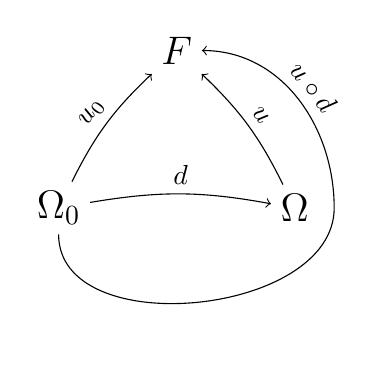
\begin{tikzpicture}
            \draw (-1.5,0) node[](A) {\Large$\Omega_0$};
            \draw (1.5,0) node[](B) {\Large$\Omega$};
            \draw (0,2) node[](C) {\Large$F$};
            \draw[->] (A) to[bend left=10] node[above,sloped]{$d$} (B);
            \draw[->] (A) to[bend left=10] node[above,sloped]{$u_0$} (C);
            \draw[->] (B) to[bend right=10] node[above,sloped]{$u$} (C);
            %\draw[] plot [smooth] coordinates {(A) (2,0) (C)};
            \draw[->] (A) to[out=270, in=270] (2,0) to[out=90,in=0] node[sloped,above]{$u \circ d$} (C);
        \end{tikzpicture}
    \end{center}
\end{enumerate}

Man unterscheidet zunächst in

\begin{enumerate}
    \item[\textbullet] Merkmalsbasierte Verfahren
    \item[\textbullet] Globale Verfahren
\end{enumerate}

\subsection{Merkmalsbasierte Verfahren}

Hierbei sollen endlich viele \mim{Landmarks}(\mim{Merkmale}) aus $u_0$ und $u$ paarweise in Einklang gebracht werden, hierraus erhält man endlich viele Gleichungen zur Schätzung von $d$. Diese Kontrollpunkte müssen jedoch vorher von Hand bestimmt werden und in den beiden gegebenen Bildern miteinander identifiziert werden, es ist nur schwer möglich dem Computer das Finden dieser Kontrollpunkte beizubringen.

Beispiel.: $d:\R^2 \to \R^2$ linear + Translation, d.h.:

\[ d:\underbrace{\mat{x_1 \\ x_2}}_{p} \mapsto \mat{a & b \\ c & d} \C \mat{x_1 \\ x_2}+ \mat{e\\f} \coloneqq \underbrace{\mat{y_1 \\ y_2}}_{q} = \mat{ax_1 + bx_2 +e\\ cx_1 + dx_2 + f} = \underbrace{\mat{x_1 & x_2 & 0 & 0 & 1 & 0\\ 0 & 0 & x_1 & x_2 & 0 & 1}}_{A_p}\C \mat{a\\b\\c\\d\\e\\f}\]

Die zu lösende Gleichung ergibt sich somit zu:

\[A_p \C \mat{a\\b\\c\\d\\e\\f} = q\]

Sind $p_1,...,p_n \in \Omega_0$ und $q_1,...,q_n \in \Omega$ paarweise zusammen gehörende Kontrollpunkte, so kann man $a,b,c,d,e,f$ über das folgende Lineare Ausgleichsproblem schätzen.

\[ \mat{\ \boxed{A_{p_1}} \ \\ \ \boxed{A_{p_2}} \ \\ \cdots \\ \ \boxed{A_{p_n}} \ } \C \mat{a\\b\\c\\d\\e\\f} \approx \mat{\ \boxed{q_1 \vphantom{A_{p_1}}} \ \\ \ \boxed{q_2 \vphantom{A_{p_1}}} \ \\ \cdots \\ \ \boxed{q_n \vphantom{A_{p_1}}} \ }\]

Dieses kann etwa über Normalengleichungen oder QR Zerlegungen geschehen.

\begin{align*}
    n<3&\text{: unterbestimmt}\\
    n=3&\text{: fair}\\
    n>3&\text{: überbestimmt}
\end{align*}

Im selben Stil können quadratische oder höhere Deformationen berechnet werden:

\[d:\underbrace{\mat{x_1 \\ x_2}}_{p} \mapsto \mat{ax_1^2 + b x_1 x_2 + c x_2^2 + d x_1 + e x_2 +f\\ g x_1^2 + hx_1x_2 + ix_2^2 + jx_1 + hx_2 +l} = \underbrace{\mat{y_1\\y_2}}_{q}\]

\[\left(
    \begin{array}{*{12}c}
        x_1^2 & x_1x_2 & x_2^2 & x_1 & x_2 & 1 & 0 & 0 & 0 & 0 & 0 & 0\\
        0 & 0 & 0 & 0 & 0 & 0 & x_1^2 & x_1x_2 & x_2^2 & x_1 & x_2 & 1
    \end{array}
    \right) \C \mat{a\\ \vdots \\ l}\]

Um die 12 gesuchten Parameter hier $a,b, ... ,l$ zu bestimmen werden $n \geq 6$ Kontrollpunkte auf jeder Seite benötigt.

Es gibt auch noch einen anderen Spezialfall der affin-linearen Deformationen, etwa über Dreh-Spiegelungen mit Verschiebung:

\[d: \mat{x_1\\x_2} \mapsto r \C \mat{cos(\varphi) & -sin(\varphi)\\ sin(\varphi) & cos(\varphi)} + \mat{e\\f}=\mat{y_1\\y_2}\]

\[\Rightarrow \mat{y_1\\y_2} = \mat{r \C cos(\varphi)x_1 -r \C sin(\varphi)x_2 + e\\ r \C sin(\varphi)x_1 + r \C cos(\varphi) x_2 + f} = \mat{x_1 & -x_2 & 1 & 0\\ x_2 & x_1 & 0 & 1} \mat{r \C cos(\varphi)\\ r \C sin(varphi)\\e \\ f} \begin{array}{c}
     \coloneqq g\\ \coloneqq h\\ \ \\ \
\end{array}\]

Somit brauchen wir $n \geq 2$ Kontrollpunkte um $g,h,e,f$ zu bestimmen, hierraus können dann $r \coloneqq \sqrt{g^2+h^2}$ und $\varphi=arctan(\frac{h}{g})$ bestimmt werden.

\subsection{Globale Verfahren}

Globale Verfahren benutzen keine Manuell bestimmten Kontrollpunkte und können somit komplett durch einen Computer durchgeführt werden, wiederum wird dieses Problem mittels der Variationsrechnung formuliert.
Hierbei lautet das zu minimierende Funktional:

\[J(d) \coloneqq \underbrace{D(u_0,u \circ d)}_{\text{\small Datenterm}} + \lambda \underbrace{R(d)}_{\text{\small Regularitätsterm}} \to \ min\]

\begin{enumerate}
    \item Wahl des Datenterms $D$
    \begin{enumerate}
        \item Punktweise Differenz in der$L^1$-Norm:
            \[D(f,g)  \coloneqq  \norm{f-g}_2^2 = \int_\Omega \abs{f(x)-g(x)}^2 dx\]
        \item Vergleich der Grauwert-Verläufe
            \[\bar{f}  \coloneqq \ \frac{1}{\abs{\Omega}} \int_\Omega f(x) dx, \quad \bar{g}  \coloneqq  \frac{1}{\abs{\Omega}} \int_\Omega g(x) dx\]
            und dann Vergleich von
            \[\frac{f - \bar{f}}{\norm{f-\bar{f}}_2} \quad \text{und} \quad \frac{g - \bar{g}}{\norm{g-\bar{g}}_2}\]
            über:
            \[\skprod{\frac{f - \bar{f}}{\norm{f-\bar{f}}_2}}{\frac{g - \bar{g}}{\norm{g-\bar{g}}_2}} \in [-1,1]\]

            \begin{enumerate}
                \item[1] bedeutet vollständige Korreliertheit mit gleicher Tendenz
                \item[-1] vollständige Korreliertheit mit entgegengesetzter Tendenz
                \item[0] bedeutet Unkorreliertheit
            \end{enumerate}

            Der sich ergebende Datenterm lautet:

            \[D(f,g)  \coloneqq  \skprod{\frac{f - \bar{f}}{\norm{f-\bar{f}}_2}}{\frac{g - \bar{g}}{\norm{g-\bar{g}}_2}}\]

            Diese Verfahren nennt sich \mim{Normalized Crosscorrelation}.
            \item Punktweise Differenzen der Gradienten:
                \[D(f,g)  \coloneqq  \norm{\nabla f - \nabla g}_2^2 = \int_\Omega \abs{\nabla f - \nabla g}^2 dx\]

            \item Vergleich der Gradientenverläufe, also NCC (wie in (b)) von $\nabla f$ und $\nabla g$.
    \end{enumerate}
    Es ist zu bemerken das (a) keine Verschiebung um eine konstante Erkennt, (b) findet sogar Transformationen der Form $f=a*g+c$.

    \item Notwendigkeit und Wahl des Regularitätsterms.
    Betrachte etwa $\begin{tabular}{|c|c|c|c|}
        \hline
        1 & 2 & 3 & 4\\
        \hline
    \end{tabular} \to \begin{tabular}{|c|c|c|c|}
        \hline
        1 & 4 & 3 & 2\\
        \hline
    \end{tabular}$, diese Zerreißung muss bestraft werden.
    Ansätze:
    \[d: \mat{x_1 \\ x_2 } \mapsto \mat{y_1(x_1,x_2) \\ y_2(x_1,x_2)}\]
    \begin{enumerate}
        \item Große Streckungen/Deformationen bestrafen
            \[R(d)  \coloneqq  \int_\Omega\bigl( \abs{\nabla y_1(x)}^2 + \abs{\nabla y_2(x)}^2   \bigr) dx \]
            Hier werden Abbleitung 1. Ordnung benutzt.
        \item Große Krümmungen bestrafen
            \[R(d)  \coloneqq  \int_\Omega\bigl( \abs{\Delta y_1(x)}^2 + \abs{\Delta y_2(x)}^2   \bigr) dx \]
            Hier werden Abbleitung 2. Ordnung benutzt.\\

            Es können aber auch Ableitungen höherer Ordnungen sowie Kombinationen verwendet werden.
    \end{enumerate}
\end{enumerate}

